C++17帶來了重要修改和幾個與併發相關的調整,先讓快速討論一下後者。在C++11中引入的\texttt{std::lock()}現在有一個相應的RAII對象,\texttt{std::scoped\_lock}。添加了共享互斥鎖\texttt{std::shared\_mutex},或者稱為讀寫互斥鎖(同樣,匹配POSIX相應的特性)。只要線程不需要獨佔訪問鎖定的資源,這個互斥鎖允許多個線程同時進行操作。這樣的線程執行只讀操作,而寫線程需要獨佔訪問,因此稱為\textbf{讀寫鎖}。理論上講,這是一個聰明的想法,但大多數實現的性能都很糟糕。

值得注意的是一個新特性,允許決定L1緩存的緩存行大小,\texttt{std::hardware\_destructive\_\linebreak interference\_size}和\texttt{std::hardware\_constructive\_interference\_size}。這些常量有助於創建緩存優化的數據結構,避免錯誤共享。

現在來看看C++17的主要新特性——\textbf{並行算法},STL算法現在有了並行版本(總的來說,這組並行算法通常稱為並行STL)。例如,下面是對\texttt{std::for\_each}的使用:

\begin{lstlisting}[style=styleCXX]
std::vector<double> v;
… add data to v … 
std::for_each(v.begin(), v.end(),[](double& x){ ++x; });
\end{lstlisting}

在C++17中,可以讓標準庫在可用的處理器上並行執行:

\begin{lstlisting}[style=styleCXX]
std::vector<double> v;
… add data to v … 
std::for_each(std::execution::par,
			v.begin(), v.end(),[](double& x){ ++x; });
\end{lstlisting}

並行版本的STL算法有一個新的第一個參數:執行策略。注意,執行策略不是單個類型,而是一個模板參數。該標準提供了幾個執行策略,前面使用的並行策略\texttt{std::execution::par},允許算法在多個線程上執行。線程的數量和線程中計算分區的方式沒有指定的,完全取決於實現。順序策略\texttt{std::execution::seq}則是在單個線程上執行算法,與不使用任何策略(或在C++17之前)執行算法的方式相同。

還有一個並行的非串行策略,\texttt{std::execution::par\_unseq}。這兩個並行策略之間有微妙的區別,理解這個區別很重要。標準表示無序策略允許在單個線程中交叉進行計算,從而允許進行其他優化,如向量化。但優化編譯器在生成機器碼時可以使用像AVX這樣的向量指令,而且這無需任何來C++代碼的幫助。編譯器只是找到向量化的機會,並將常規的單字指令替換為向量指令。那這裡有什麼不同呢?

為了理解非串行策略的本質,必須考慮一個更復雜的例子。現在,不是簡單地操作每個元素,想使用共享數據做一些計算:

\begin{lstlisting}[style=styleCXX]
double much_computing(double x);
std::vector<double> v;
… add data to v … 
double res = 0;
std::mutex res_lock;
std::for_each(std::execution::par, v.begin(), v.end(),
[&](double& x){ 
	double term = much_computing(x);
	std::lock_guard guard(res_lock);
	res += term;
});
\end{lstlisting}

這裡對每個向量元素進行一些計算,然後累加結果的總和。計算本身可以並行完成,但是累加值必須由一個鎖來保護,因為所有線程都會增加同一個共享變量\textit{res}。由於鎖並行執行策略是安全的,但不能在這裡使用無順序的策略。如果同一個線程要同時處理多個向量元素(交叉處理),可能會多次嘗試獲取同一個鎖,這是會產生死鎖。如果線程持有鎖,並試圖再次鎖定它,第二次嘗試將會阻塞,並且線程不能繼續運行到它應該解鎖的地方。標準調用代碼(如上一個例子中的\textbf{向量化不安全})聲明,此類代碼不應與無序策略一起使用。 

既然已經瞭解了並行算法在理論上是如何工作的,那麼在實踐中呢?簡短的回答很好,但有一些瑕疵,還是來看看完整的版本。

檢查並行算法之前,必須準備構建的環境。要編譯C++程序只需要安裝所需的編譯器版本,比如GCC,然後就可以了,但並行算法卻不是這樣。在寫這本書的時候,安裝過程有些繁瑣。

最新的GCC和Clang版本都包含了並行的STL頭文件(在一些安裝中,Clang需要安裝GCC,因為它使用GCC提供的並行STL),這個問題出現在較底的層次上。這兩個編譯器使用的運行時線程系統是Intel的\textbf{threading Building Blocks (TBB)},這兩個編譯器都沒有在安裝中包含TBB。麻煩的是,編譯器的每個版本都需要對應的TBB版本,舊版本和新版本都不能工作(錯誤會在編譯和鏈接時出現)。要運行與TBB鏈接的程序,可能需要將TBB庫添加到庫路徑中。

當解決了這些問題,並配置了編譯器和必要的庫,使用並行算法並不比使用其他STL困難。那麼其擴展性怎麼樣?我們可以做一些基準測試。 

從\texttt{std::for\_each}開始,沒有鎖,並且每個元素都需要大量的計算(函數\texttt{work()}非常耗時,精確的操作對於擴展性並不重要):

\hspace*{\fill} \\ %插入空行
\noindent
\textbf{parallel\_algorithm.C}
\begin{lstlisting}[style=styleCXX]
std::vector<double> v(N);
std::for_each(std::execution::par,
v.begin(), v.end(),[](double& x){ work(x); });
\end{lstlisting}

以下是運行在兩個線程上的串行版本和並行版本的性能:

%\hspace*{\fill} \\ %插入空行
\begin{center}
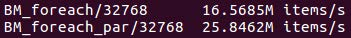
\includegraphics[width=0.9\textwidth]{content/2/chapter8/images/1.jpg}\\
圖8.1 - 並行\texttt{std::foreach}在2個cpu上的基準測試
\end{center}

擴展性還不錯。注意,向量大小N相當大,有32K個元素。對於更大的向量,擴展效果確實有所改善。但是,對於相對較小的數據量,並行算法的性能很差:

%\hspace*{\fill} \\ %插入空行
\begin{center}
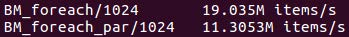
\includegraphics[width=0.9\textwidth]{content/2/chapter8/images/2.jpg}\\
圖8.2 - 短序列並行\texttt{std::foreach}的基準測試
\end{center}

對於包含1024個元素的向量,並行版本比串行版本慢。原因是執行策略在每個並行算法開始時啟動所有線程,並在結束時回收它們。啟動新線程需要花費大量時間,因此當計算時間較短時,開銷會超過我們從並行化中獲得的任何加速。這不是標準強加的要求,而是當前GCC和Clang中並行STL的實現管理其與TBB系統交互的方式。 

當然,並行算法提高性能的大小取決於硬件、編譯器,及其並行性的實現,以及每個元素的計算量。例如,可以嘗試逐元素計算:

\begin{lstlisting}[style=styleCXX]
std::for_each(std::execution::par,
v.begin(), v.end(),[](double& x){ ++x; });
\end{lstlisting}

現在,處理32k元素數組,並行性並沒有優勢:

%\hspace*{\fill} \\ %插入空行
\begin{center}
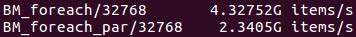
\includegraphics[width=0.9\textwidth]{content/2/chapter8/images/3.jpg}\\
圖8.3 - 並行\texttt{std::foreach}的基準測試,以實現每個元素的快速計算
\end{center}

對於更大的數組,並行算法可能會有優勢,除非內存訪問速度限制了單線程和多線程版本的性能(這是一個很大的內存限制計算)。

也許更令人印象深刻的是那些很難並行化算法的性能,比如\texttt{std::sort}:

\begin{lstlisting}[style=styleCXX]
std::vector<double> v(N);
std::sort(std::execution::par, v.begin(), v.end();
\end{lstlisting}

輸出:

%\hspace*{\fill} \\ %插入空行
\begin{center}
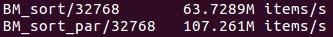
\includegraphics[width=0.9\textwidth]{content/2/chapter8/images/4.jpg}\\
圖8.4 - 並行\texttt{std::sort}的基準測試
\end{center}

同樣,在並行算法生效之前,需要足夠大的數據量(對於1024個元素,單線程排序更快)。排序並不是容易並行化的算法,而且在雙精度浮點數(比較和交換)上對每個元素進行的計算非常快。儘管如此,並行算法展示了非常好的加速,如果元素比較的代價更高,性能會變得更好。 

並行STL算法如何與線程交互?若在兩個線程上同時運行兩個並行算法會發生什麼?首先,與在多線程上運行的代碼一樣,必須確保線程安全(無論使用哪種排序,在同一個容器上並行兩個排序不個好主意)。除此之外,還會發現多個並行算法可以共存,但無法控制調度系統,它們都試圖在可用的CPU上運行,因此會出現爭奪資源。根據每個算法的擴展性,並行運行幾個算法可能會獲得更高的總體性能,也可能不會。

總的來說,當STL算法運行在足夠大的數據量上時,其並行版本的性能非常好,儘管足夠大的數據量取決於特定的計算。可能需要額外的庫來編譯和運行使用並行算法的程序,配置這些庫可能需要一些工作量。而且,並不是所有的STL算法都有並行版本(例如,\texttt{std::accumulate}就沒有)。

……

現在我們可以在穿梭時間,直接跳到C++20。














